\subsection{Auswertung}
Bei der Analyse des vorgegebenen Pulvers mittels Debye Scherrer Verfahren ergab sich das Diffraktogramm in Abb. \ref{fig:diffr_pulver}.
Zum Vergleich sind Diffraktogramme von Silicium und Germanium (Abb. \ref{fig:diffr_sil_sim} und Abb. \ref{fig:diffr_ger_sim}) simuliert worden. Man sieht sofort, dass das Diffraktogramm von Silicium mit dem der untersuchten Probe sehr gut �bereinstimmt. Daneben stellt man einen Offset der simulierten Daten zu den gemessenen fest. Um diesen Offset zu bestimmen, wurde an alle drei Datens�tze ein Multivoigt gefittet. Die Voigtverteilung wird dabei numerisch approximiert, wobei die in Python bereits implementierte Voigt-Verteilung aus der Bibliothek "`lmfit"' verwendet wird. Der Fit an die Messdaten passt mit einem reduzierten Chiquadrat von 22,335 relativ gut, wenn man beachtet, dass auch bei kleineren Zahlraten ein Fehler von $\sqrt{N}$ verwendet wurde. Erstaunlicherweise passen die Fits, bei einem Fehler von $\sqrt{N}$, eher schlecht an die simulierten Daten. Man sieht aber, dass die Maxima gut getroffen werden, was in diesem Versuchsteil das wichtigste Kriterium f�r die Auswertung ist. Es ergeben sich reduzierte Chiquadrate von 562 und 19989, sodass diese Fits nicht als besonders gut betrachtet werden k�nnen. Wie die Fits in der N�he einzelner Peaks aussehen, kann im Anhang nachvollzogen werden.
Die Lage der Maxima sind in Tabelle \ref{table:mu_vergleich_pul_si_ger} dargestellt, wobei der Fehler �berall bei $\pm$1 auf der letzten angegebenen Nachkommastelle liegt. Die Fehler ergaben sich aus dem Fit, und wurden nach oben abgesch�tzt.
\begin{table}[H]
\caption{Braggreflexe vom Pulver, verglichen mit den simulierten Daten}
\label{table:mu_vergleich_pul_si_ger}
\begin{tabular}{|c|c|c|c|c|c|}
\hline  Pulver K$_{\alpha_1}$ & Pulver K$_{\alpha_2}$ & Silicium K$_{\alpha_1}$ & Silicium K$_{\alpha_2}$ & Germanium K$_{\alpha_1}$ & Germanium K$_{\alpha_2}$ \\ 
\hline 2$\theta/^{\circ}$ & 2$\theta/^{\circ}$ & 2$\theta/^{\circ}$ & 2$\theta/^{\circ}$ & 2$\theta/^{\circ}$ & 2$\theta/^{\circ}$ \\ 
\hline 28,287 & 28,363 & 28,447 & 28,521 & 27,317 & 27,389 \\ 
\hline 47,146 & 47,271 & 47,311 & 47,436 & 45,365 & 45,484 \\ 
\hline 55,963 & 56,116 & 56,134 & 56,284 & 53,768 & 53,911 \\ 
\hline 68,969 & 69,167 & 68,144 & 69,340 & 66,096 & 66,282 \\ 
\hline 76,223 & 76,454 & 76,391 & 76,615 & 72,923 & 73,133 \\ 
\hline 87,875 & 88,155 & 88,050 & 88,325 & 83,813 & 84,067 \\ 
\hline 94,802 & 95,111 & 94,975 & 95,285 & 90,214 & 90,499 \\ 
\hline 106,565 & 106,949 & 106,736 & 107,119 & 100,928 & 101,275 \\ 
\hline 113,949 & 114,388 & 114,122 & 114,563 & 107,525 & 107,915 \\ 
\hline 127,406 & 127,985 & 127,584 & 128,166 & 119,145 & 119,630 \\
\hline 136,766 & 137,505 & 136,943 & 137,671 & 126,764 & 127,335 \\
\hline 
\end{tabular}
\end{table}
Wenn man sich dazu die Diffraktogramme in den Abbildungen \ref{fig:diffr_pulver}, \ref{fig:diffr_sil_sim} und \ref{fig:diffr_ger_sim} anguckt, f�llt auf, dass das Diffraktogramm des untersuchten Pulvers mit dem simulierten Diffraktogramm von Silicium sehr gut �bereinstimmt.\\
Genauer gesagt ist das simulierte Diffraktogramm leicht nach rechts veschoben. Deshalb wurden Differenzplots, bei denen die Peaks nach der Energie von gro� nach klein geordnet sind,  erstellt (Abb. \ref{fig:differenzplot_energie}). In zwei weiteren Plots wurde zus�tzlich zwischen den Peaks K$_{\alpha_1}$, K$_{\alpha_2}$ unterschieden.(Abb. \ref{fig:differenzplot_energie_alpha_1} und \ref{fig:differenzplot_energie_alpha_2})
\begin{figure}[H]
  \centering
  \caption{Peakdifferenzen der Energie nach geordnet} 
  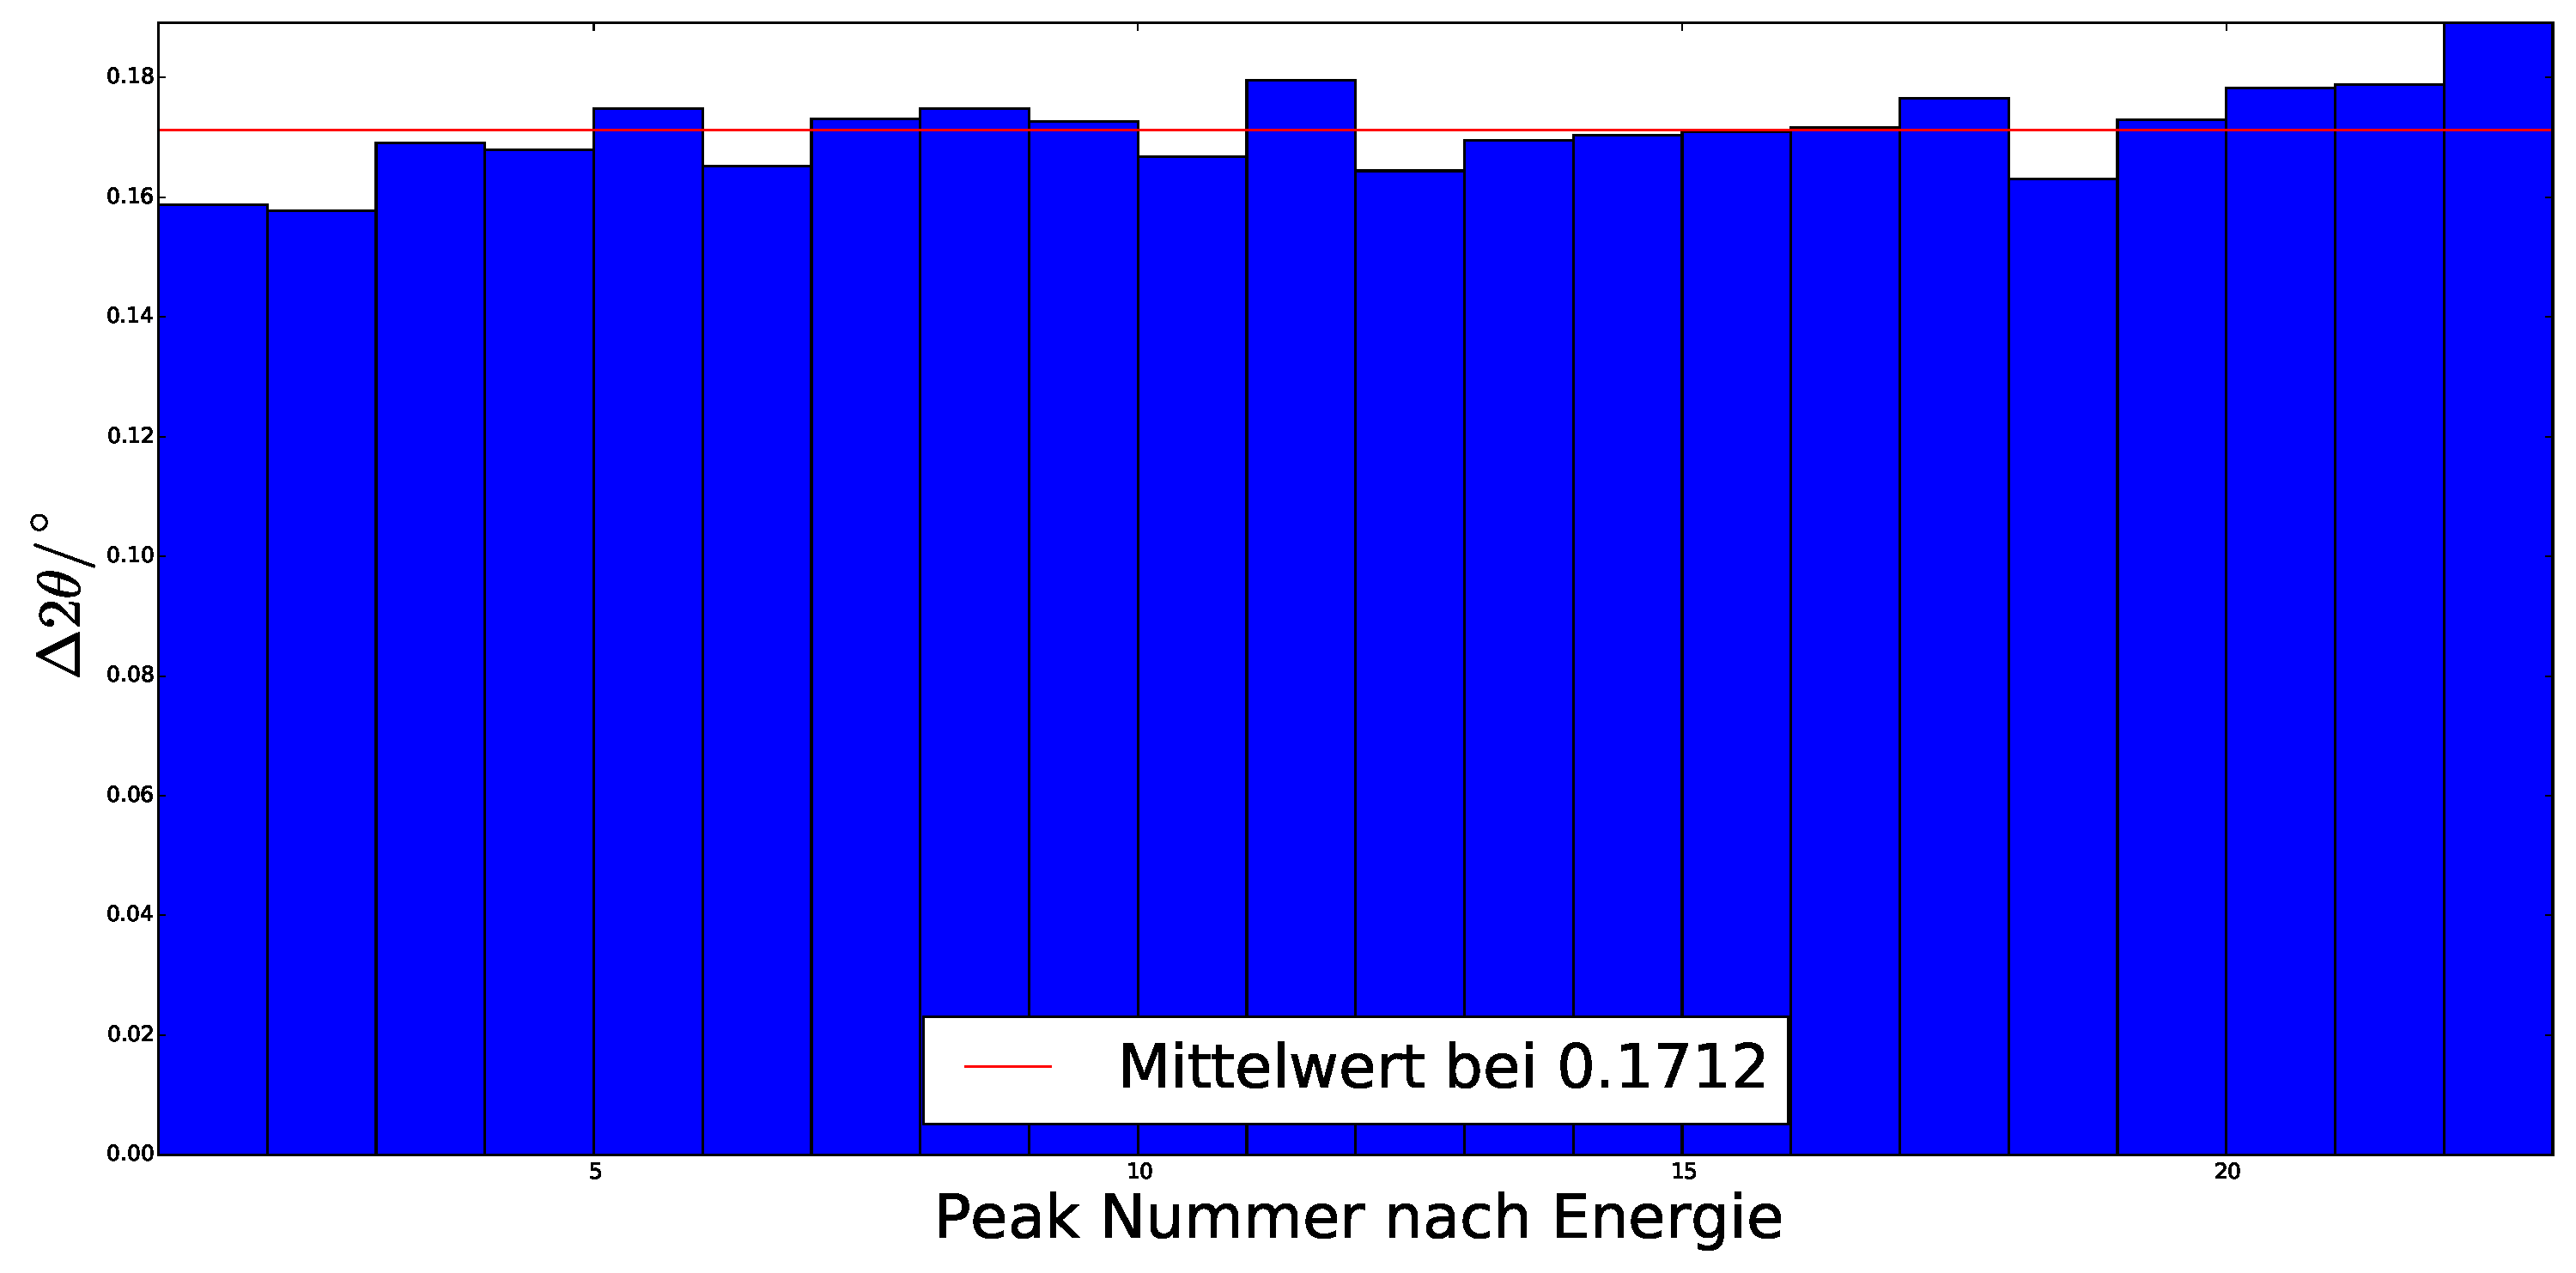
\includegraphics[scale = 0.35]{Differenzplot_pulver_Energie}
  \label{fig:differenzplot_energie}
\end{figure}
\begin{figure}[H]
\begin{minipage}{.49\textwidth}
  \centering
  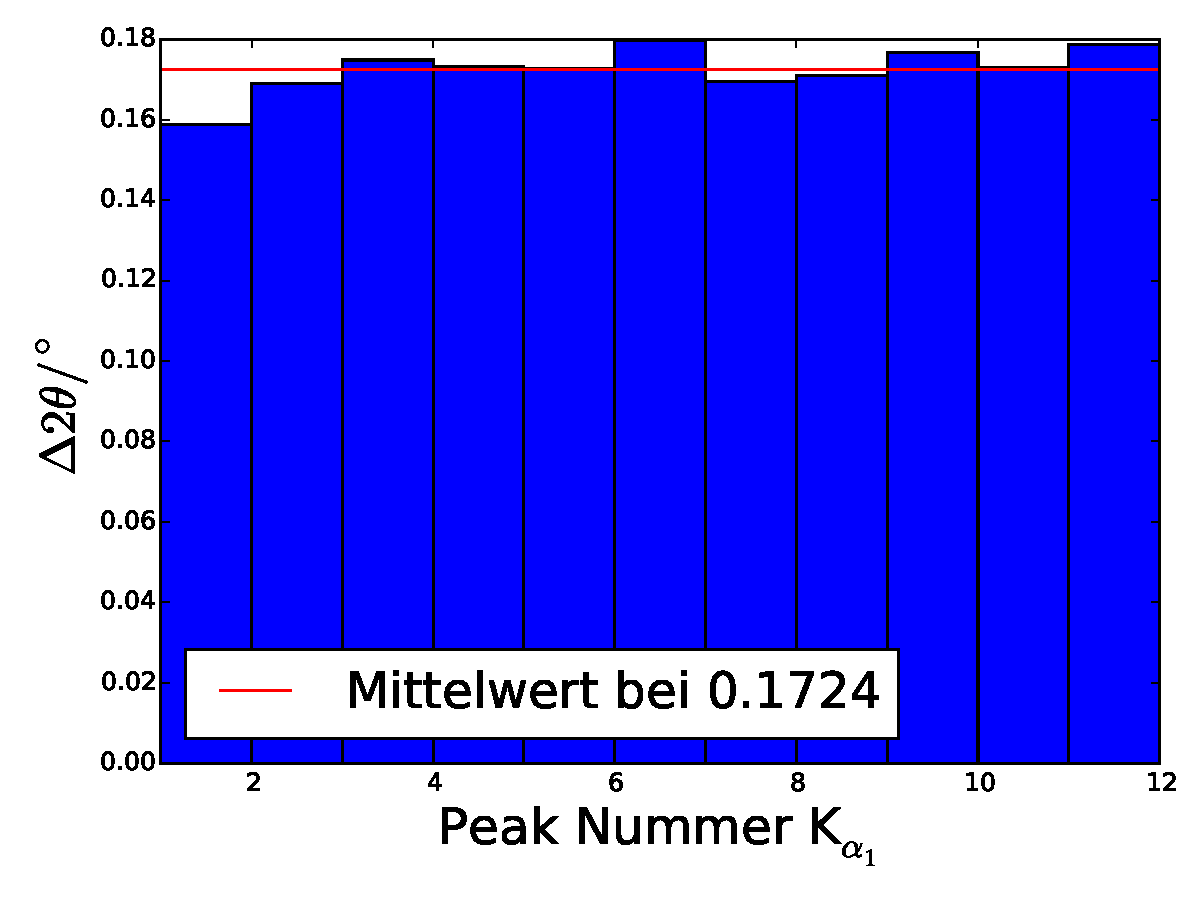
\includegraphics[scale=0.46]{Differenzplot_pulver_K_alpha_1}
  \captionof{figure}{Peakdifferenzen von K$_{\alpha_1}$ der Energie nach geordnet}
  \label{fig:differenzplot_energie_alpha_1}
\end{minipage}
\hspace{0.2cm}
\begin{minipage}{.49\textwidth}
  \centering
  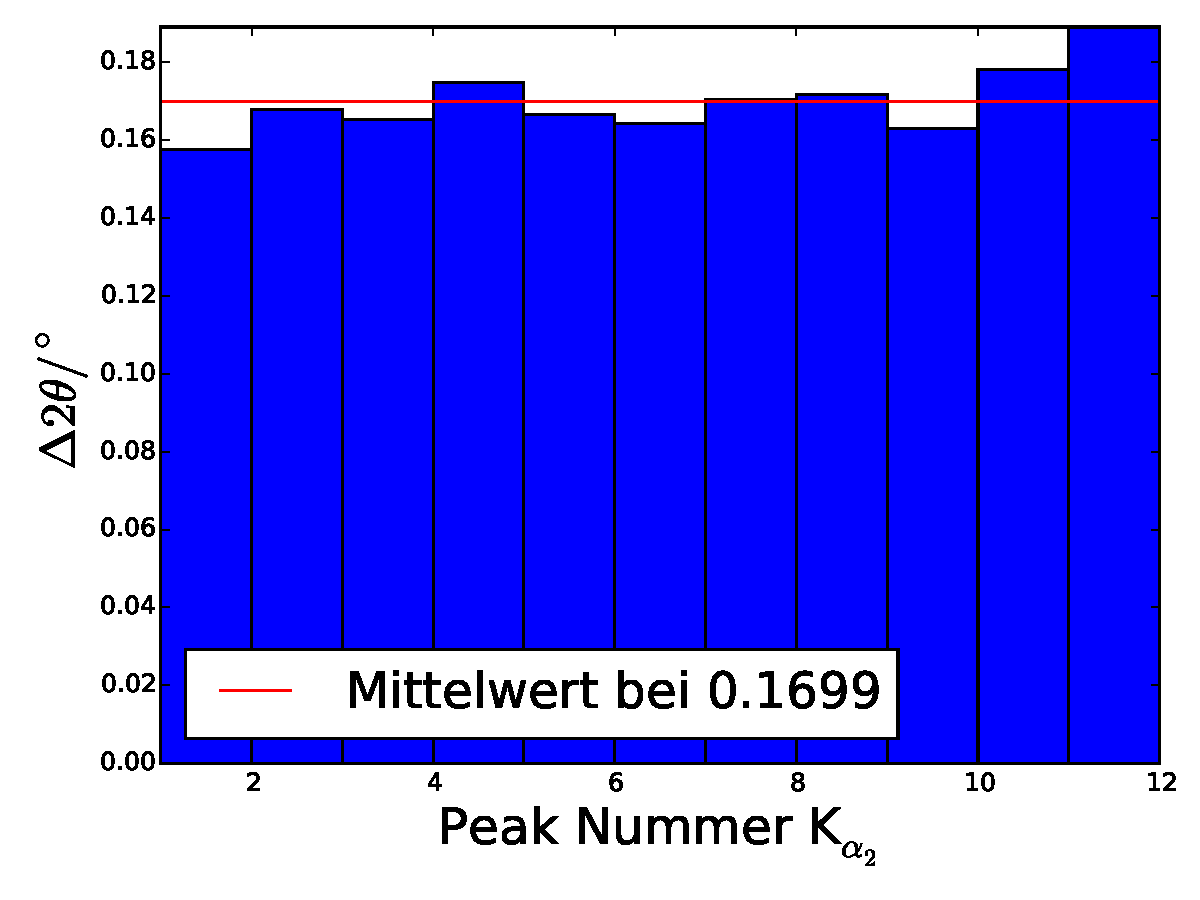
\includegraphics[scale=0.45]{Differenzplot_pulver_K_alpha_2}
  \captionof{figure}{Peakdifferenzen von K$_{\alpha_2}$ der Energie nach geordnet}
  \label{fig:differenzplot_energie_alpha_2}
\end{minipage}
\end{figure}
Man sieht bei allen Plots einen leichten Anstieg der Differenzen der Energien f�r kleine Energiewerte. Es wird trotzdem ein Offset in Form einer Konstanten angenommen. Es ergibt sich damit eine mittlere Abweichung von \SI{0.1712}{\degree}, die haupts�chlich auf einen systematischen Fehler zur�ckzuf�hren ist. Nachdem man die Messdaten um diesen Offset nach rechts verschiebt, stimmt die Lage der Peaks des untersuchten Pulvers bis auf die bereits angesprochene minimale Steigung �berein. Das untersuchte Material kann also mit Siliciumpulver identifiziert werden. Die Herkunft des Offsets ist auf die im Vergleich zur Theorie h�heren gemessenen Energien der K$_{\alpha_1}$ und K$_{\alpha_2}$ Linien in Versuchsteil 3.2.3 zur�ckzuf�hren. Indem man Formel \ref{eqn:bragg_kurze_fassung} nach $\theta$ umstellt, Tabelle \ref{tab:enerige_k}) verwendet und die Winkel mit den Winkeln, welche sich aus den Literaturwerten f�r die Energien ergeben, vergleicht, findet man schlie�lich auch einen Grund f�r die bereits angesprochene minimale Steigung. Nachdem man Formel \ref{eqn:bragg_kurze_fassung} bis zur ersten Ordnung taylort und die Differenz zwischen
\begin{align}
\sin(\theta_{Theorie}) = \frac{hc}{2d_{[nh,nk,nl]} E_{Literatur}}
\end{align}
und
\begin{align}
\sin(\theta_{Messung}) &\approx \frac{hc}{2d_{[nh,nk,nl]} E_{Messung}} \\ \notag
&= \frac{hc}{2d_{[nh,nk,nl]}}\left(\frac{1}{E_{Literatur}}-\frac{1}{E^2_{Literatur}}(E_{Messung}-E_{Literatur})\right)
\end{align}
bildet, findet man den Offset
\begin{align}
\Delta\theta \approx \sin(\theta_{Messung})-\sin(\theta_{Theorie}) \approx \frac{(-1)hc}{2d_{[nh,nk,nl]}E^2_{Literatur}}(E_{Messung}-E_{Literatur})
\end{align}
welcher abh�ngig von $d_{[nh,nk,nl]}$ ist. Bei gro�en Netzebenenabst�nden (kleinen Winkeln $\theta$) ergibt sich ein kleinerer negativer Offset, sowie bei kleinen Netzebenenabst�nden (gr��eren Winkeln $\theta$) ein gr��erer negativer Offset. Die Steigung des Offsets ist gering, da die Unterschiede zwischen den Netzebenenabst�nden gering sind.  Ein konstanter Offset ist deshalb f�r die qualitative Betrachtung ausreichend.
\begin{sidewaysfigure}
\centering
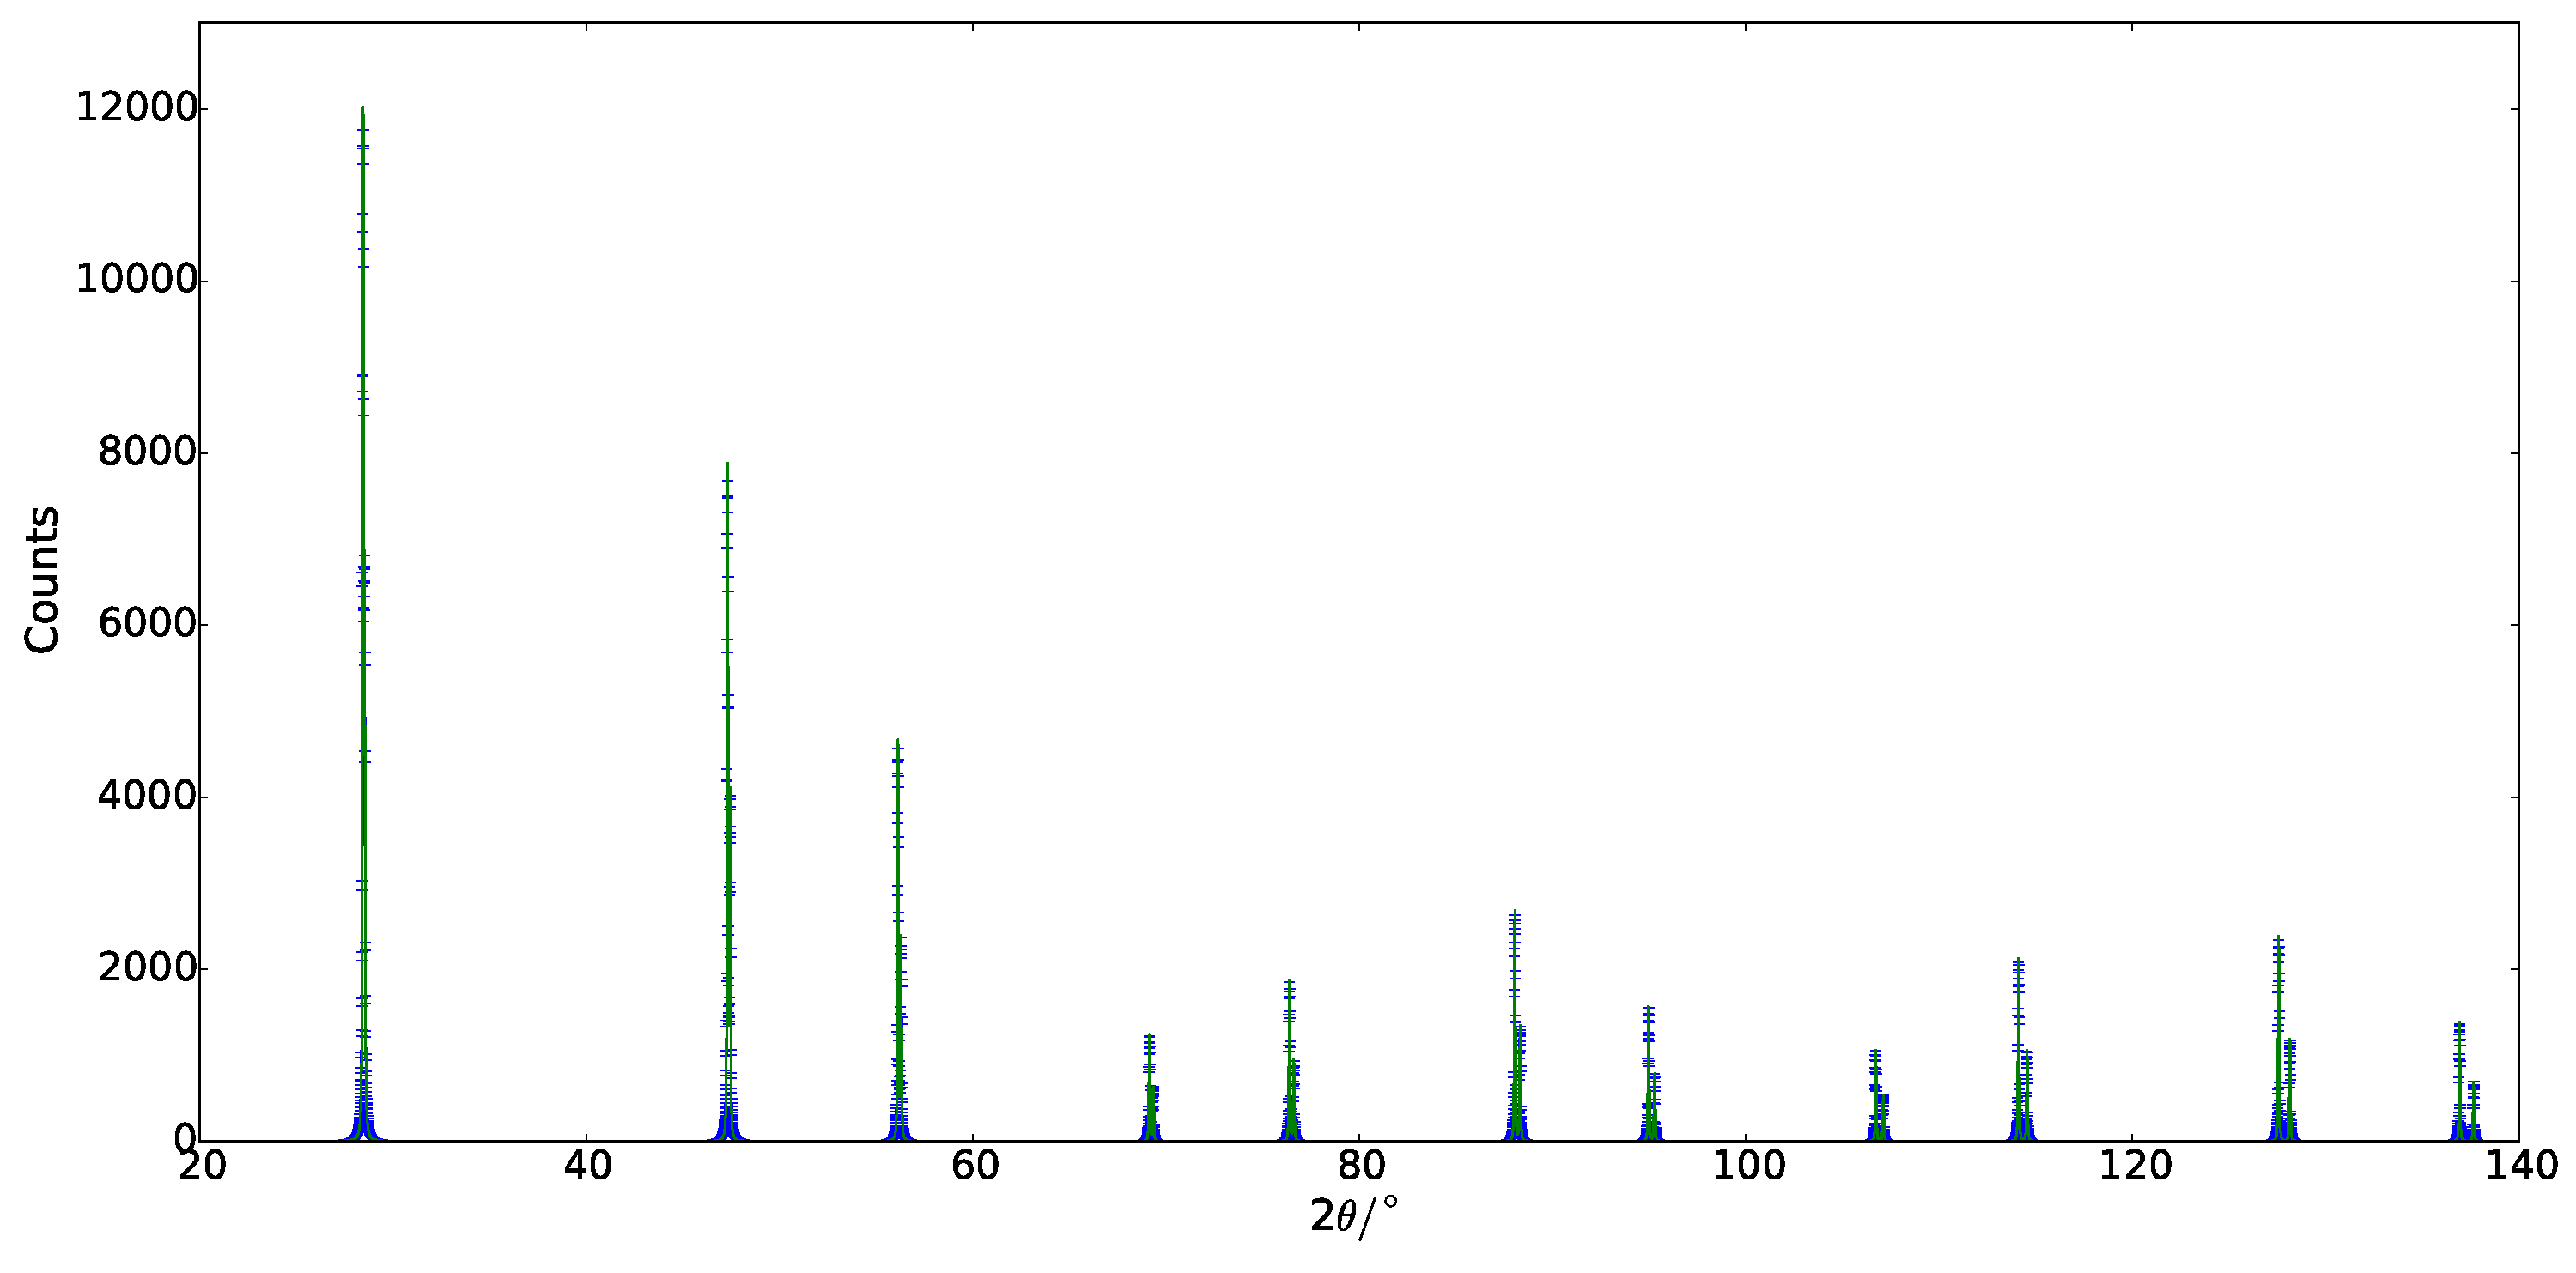
\includegraphics[width = 1.0\textwidth, height = 0.7\textwidth]{messung_pulver_ges}
\caption{Diffraktogramm der Pulverprobe}
\label{fig:diffr_pulver}
\end{sidewaysfigure}
\begin{sidewaysfigure}
\centering
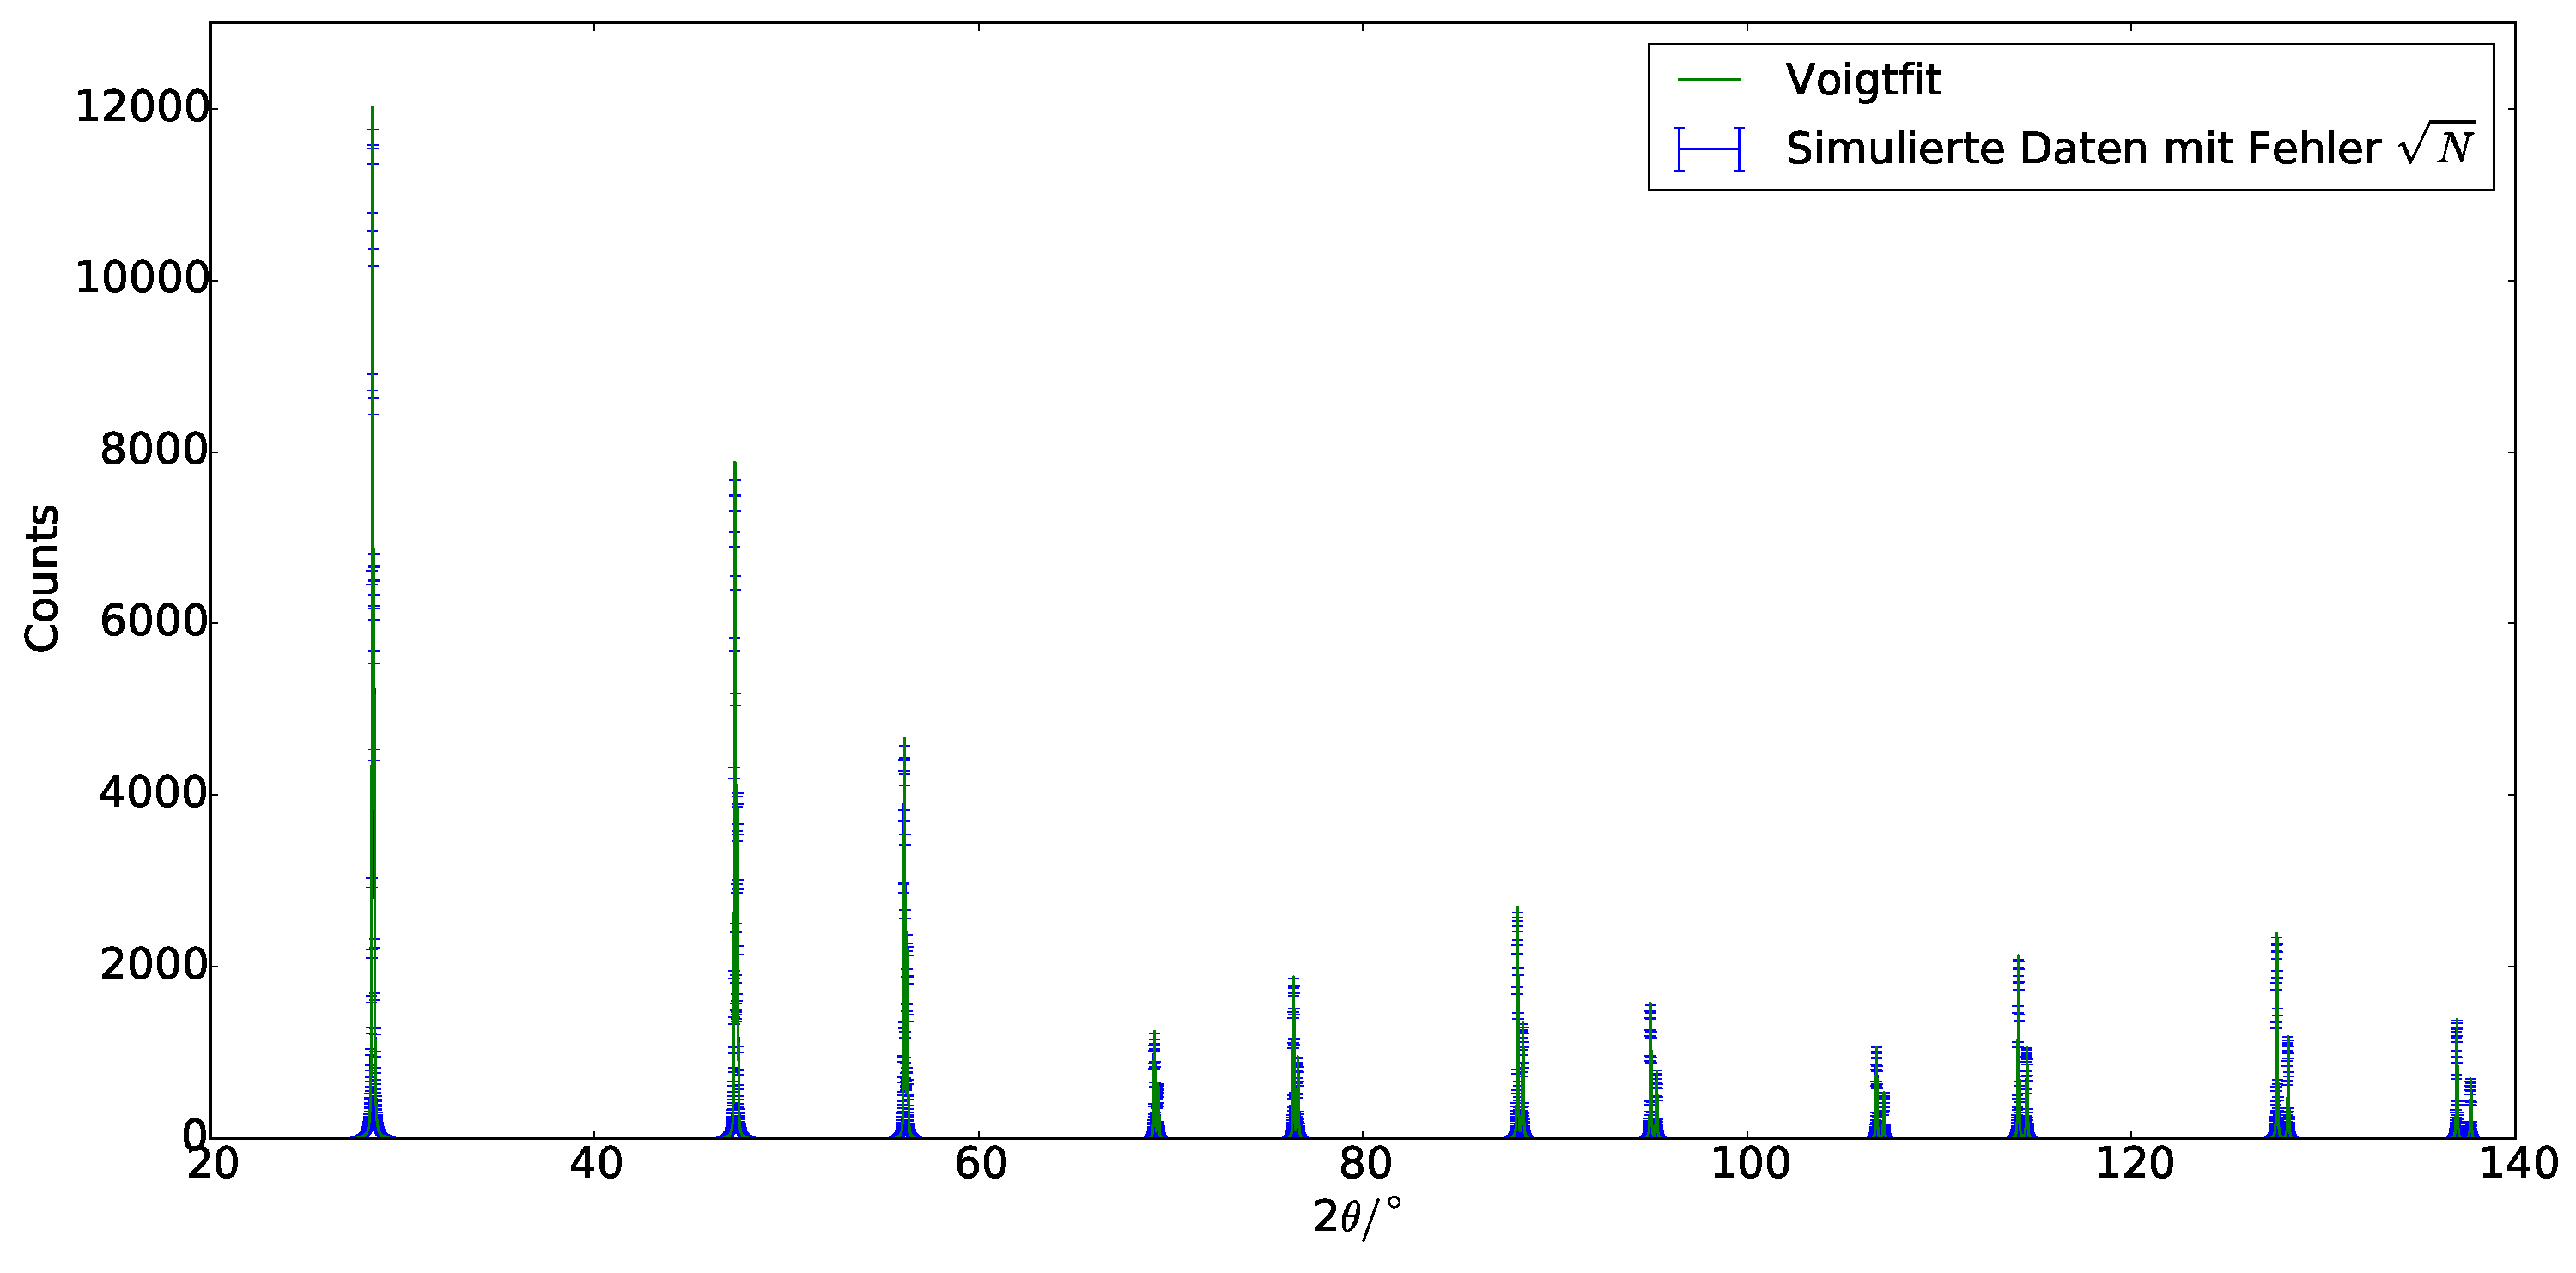
\includegraphics[width = 1.0\textwidth, height = 0.7\textwidth]{Simulation_Siliciumpulver_ges}
\caption{Diffraktogramm der Siliciumsimulation}
\label{fig:diffr_sil_sim}
\end{sidewaysfigure}
\begin{sidewaysfigure}
\centering
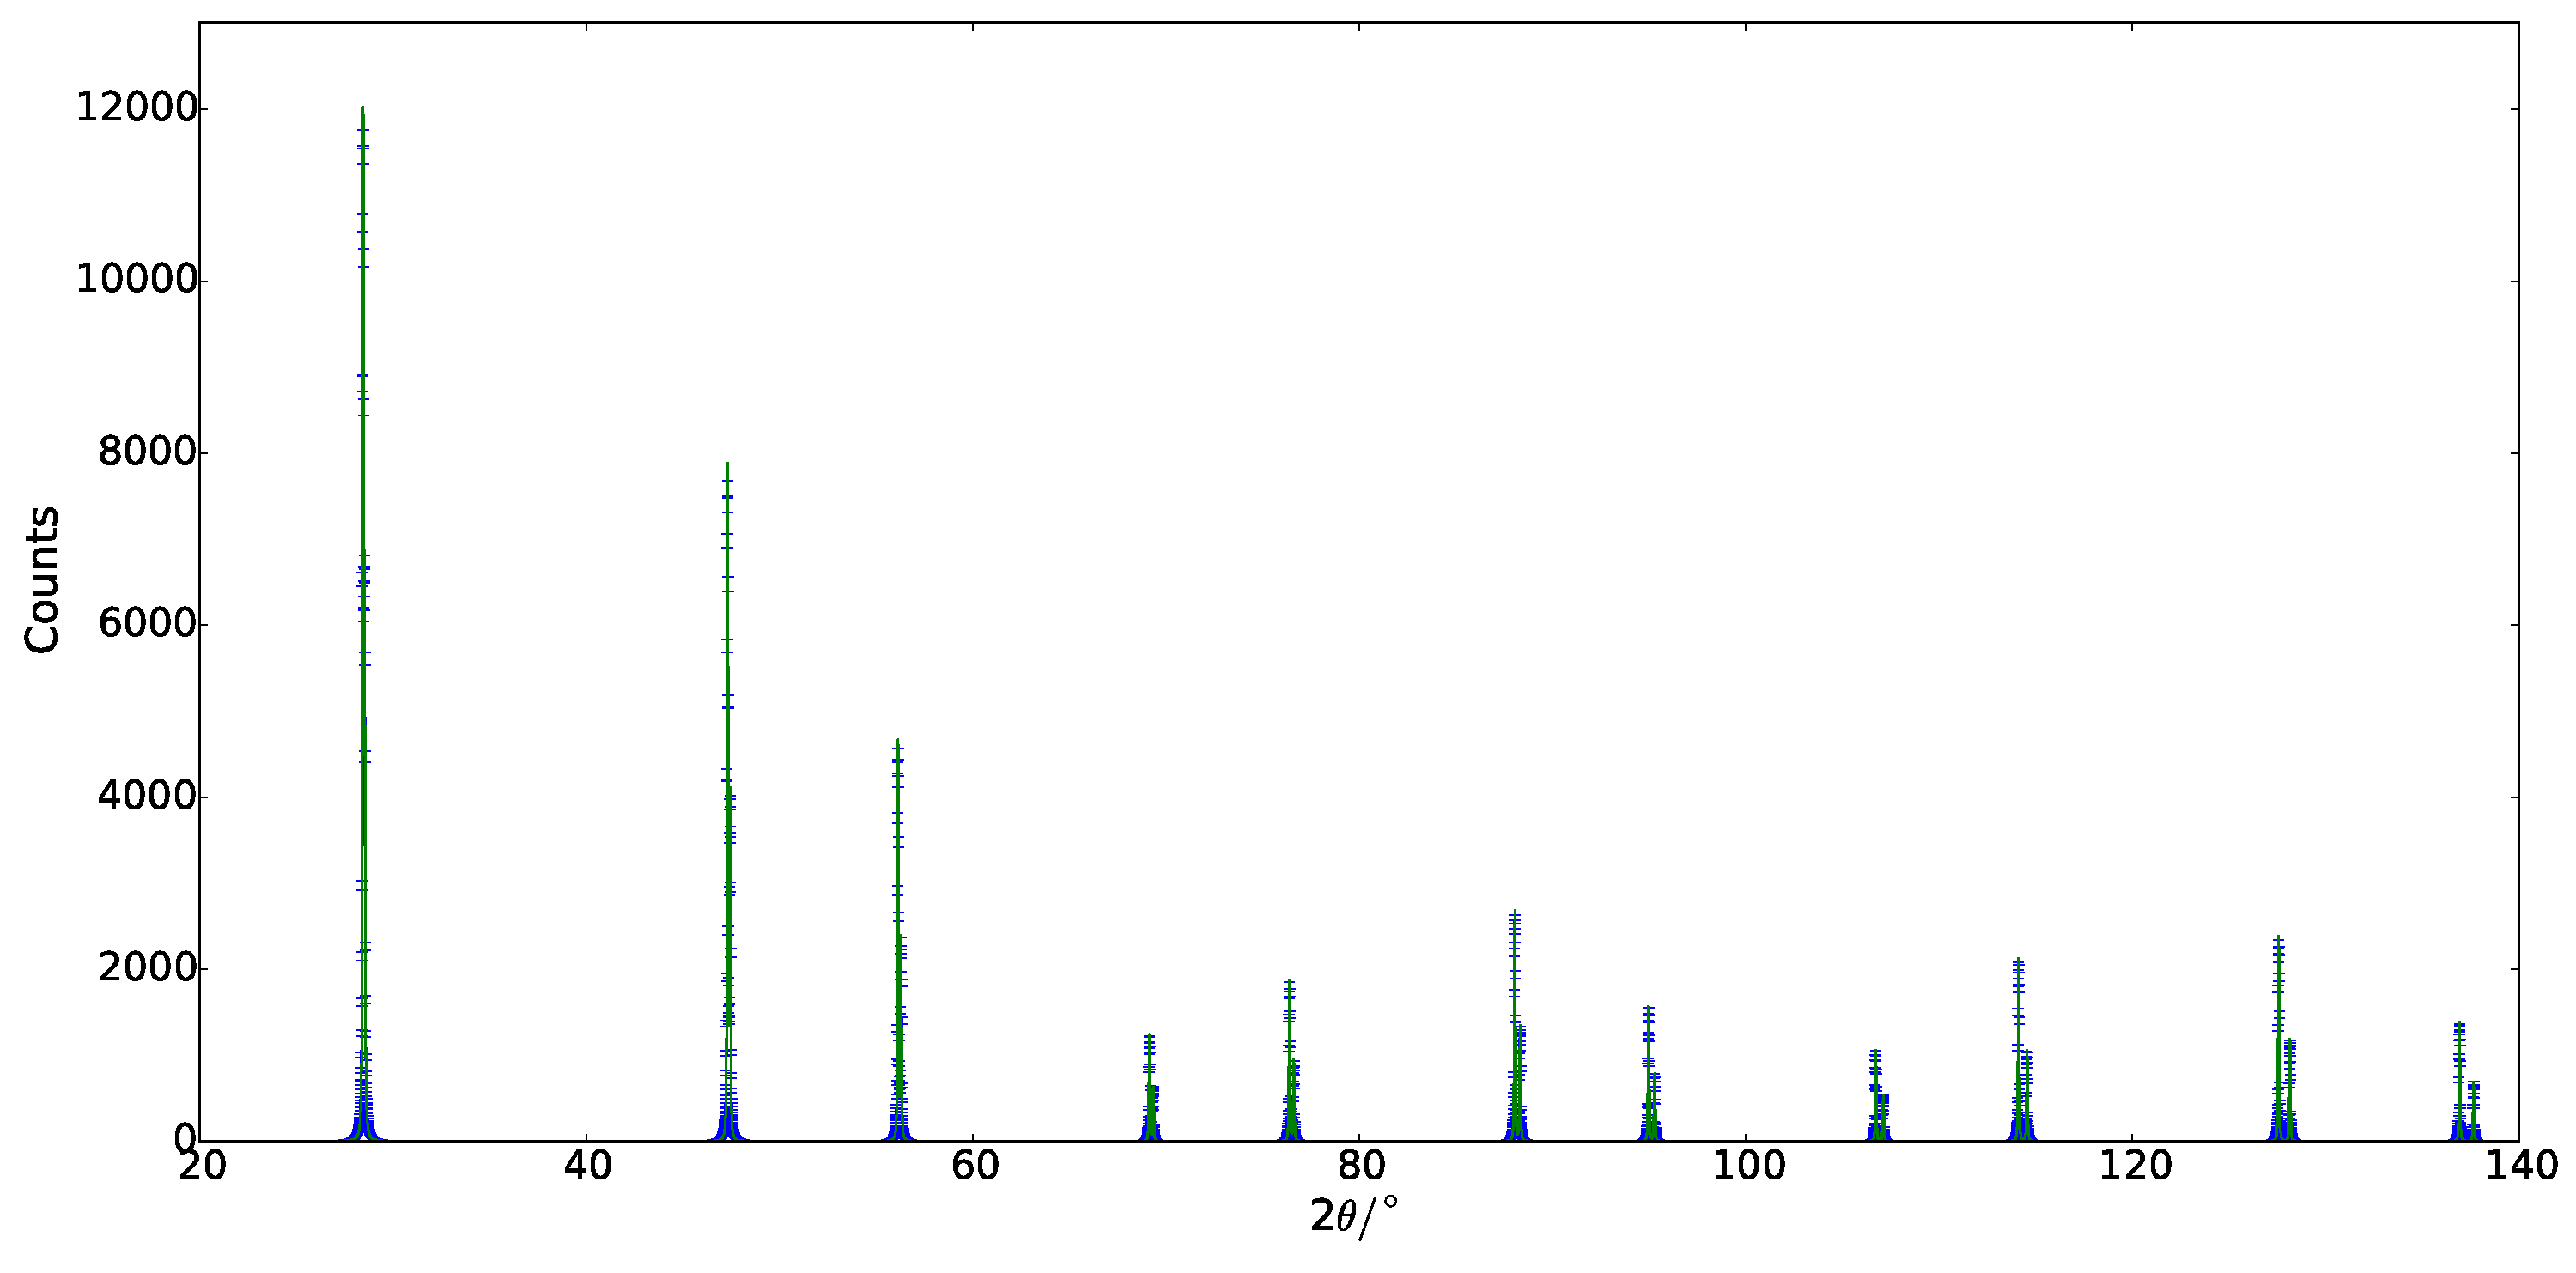
\includegraphics[width = 1.0\textwidth, height = 0.7\textwidth]{messung_pulver_ges}
\caption{Diffraktogramm der Germaniumsimulation}
\label{fig:diffr_ger_sim}
\end{sidewaysfigure}
